\documentclass[12pt]{article}
\usepackage{soul}
\usepackage{tikz}
\usepackage{amsmath}
\usepackage{amsthm}
\usepackage{amssymb}
\usepackage{lipsum}
\usepackage{float}
\usepackage{titlesec}

\usepackage[strict]{changepage} 
\usepackage{framed} 

\usepackage{enumerate}
\usepackage{subfigure}
\usepackage{geometry}
\usepackage{graphicx}
\usepackage{booktabs}
\usepackage{makecell}
\usepackage{xeCJK}
\usepackage{tcolorbox}
\usepackage[dvipsnames]{xcolor}
\setcounter{secnumdepth}{4}
\geometry{a4paper,scale=0.8}
\linespread{1}

\usepackage{pdfpages}
\renewcommand{\baselinestretch}{1.4}

\definecolor{formalshade}{rgb}{0.95,0.95,1} % 文本框颜色

\newenvironment{formal}{%
\def\FrameCommand{%
\hspace{1pt}%
{\color{Blue}\vrule width 2pt}%
{\color{formalshade}\vrule width 4pt}%
\colorbox{formalshade}%
}%
\MakeFramed{\advance\hsize-\width\FrameRestore}%
\noindent\hspace{-4.55pt}% 
\begin{adjustwidth}{}{7pt}%
\vspace{2pt}\vspace{2pt}%
}
{%
\vspace{2pt}\end{adjustwidth}\endMakeFramed%
}

\newcounter{mytheoremcounter}
\newcounter{mydefinitioncounter}
\newcounter{mylemmacounter}
%theorem
\newtcolorbox{mytheorem}[1][]{
    colback=blue!5!white,      
    colframe=Blue,    
    fonttitle=\bfseries,       
       title=Theorem~\refstepcounter{mytheoremcounter}\themytheoremcounter,  
    label=#1                 
}
%definition
\newtcolorbox{mydefinition}[1][]{
    colback=SpringGreen!5!white,     
    colframe=SpringGreen!88!black,     
    fonttitle=\bfseries,       
       title=Definition~\refstepcounter{mydefinitioncounter}\themydefinitioncounter,  
    label=#1                    
}

\newtcolorbox{mylemma}[1][]{
    colback=blue!5!white,     
    colframe=Blue,  
    fonttitle=\bfseries,       
       title=Lemma~\refstepcounter{mylemmacounter}\themytheoremcounter, 
    label=#1                   
}

\titleformat{\section}
  {\large\bfseries}
  {\thesection}    
  {1em}           
  {}               

\newtheorem{theorem}{Theorem}[section]
\newtheorem{definition}{Definition}[section]
\newtheorem{corollary}{Corollary}[theorem]
\newtheorem{lemma}[theorem]{Lemma}

\begin{document}
\begin{center}
\begin{large}
\textbf{Approximation by Superpositions of a Sigmoidal Function}\\
\end{large}
神经网络的万能近似定理
\end{center}

1989年,Cybenko 发表了一篇题为《Approximation by Superpositions of a Sigmoidal Function》的论文。在这篇论文中,Cybenko 证明了具有单一隐藏层的前馈神经网络可以逼近任何在紧集上定义的连续函数,这一结论后来被称为万能逼近定理 \textbf{Universal Approximation Theorem}。在这篇文章中,我会试着梳理整个证明的流程,澄清一些我在阅读中遇到的困惑点,并对 Cybenko 略过的细节作更深入的数学说明。以下内容会涉及许多测度论与泛函分析的内容,但是并不艰深,相信没有基础也能够参透证明的精髓。

\section{问题描述}

\begin{figure}[H]
    \centering
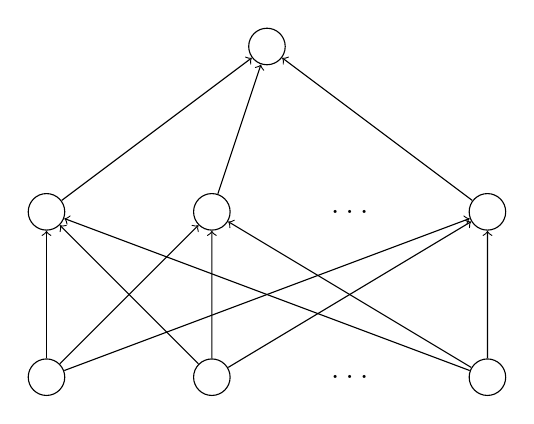
\begin{tikzpicture}[scale=1.4, every node/.style={scale=1.4}]

    \node[circle, draw] (input1) at (0, 0) {};
    \node[circle, draw] (input2) at (1.5, 0) {};
    \node[circle, draw] (input3) at (4, 0) {};
    
    \node[circle, draw] (hidden1) at (0, 1.5) {};
    \node[circle, draw] (hidden2) at (1.5, 1.5) {};
    \node[circle, draw] (hidden3) at (4, 1.5) {};
    \node[circle, draw] (output1) at (2, 3) {};
    
    \node at (2.75, 0) {\scriptsize \(\dots\)};
    \node at (2.75,1.50) {\scriptsize \(\dots\)};
    
    \draw[->] (input1) -- (hidden1);
    \draw[->] (input1) -- (hidden2);
    \draw[->] (input1) -- (hidden3);
    
    \draw[->] (input2) -- (hidden1);
    \draw[->] (input2) -- (hidden2);
    \draw[->] (input2) -- (hidden3);
    
    \draw[->] (input3) -- (hidden1);
    \draw[->] (input3) -- (hidden2);
    \draw[->] (input3) -- (hidden3);
    
    \draw[->] (hidden1) -- (output1);
    \draw[->] (hidden2) -- (output1);
    \draw[->] (hidden3) -- (output1);
    
    \end{tikzpicture}
\end{figure}

单隐藏层的前馈神经网络通常有如下形式
\begin{align*}
    \sum_{j=1}^N \alpha_j \sigma (w_j^T x +\theta_j).
\end{align*}

对应到神经网络的结构上,$w_j$ 是作用于输入 $x$ 的权重,$\alpha_i$ 是隐藏层输出的权重,$\theta_i$ 是神经元 $i$ 的偏置。我们称 $w_j^Tx+\theta_j$ 为关于神经网络输入的仿射变换 (affine transformaton)。\\

使 $I_n$ 为 $n$ 维单位立方体 $[0,1]^n$,在 $I_n$ 上的连续函数空间记作 $C(I_n)$,有限的常规 Borel 测度空间在 $I_n$ 上记作 $M(I_n)$。我们用 $\left\lVert f\right\rVert $ 来表示 $f\in C(I_n)$ 的一致范数,$\left\lVert \cdot\right\rVert $ 经常用来表示定义域上函数的最大值。以下证明的主要目标为,在何种条件下形为
\begin{align*}
    G(x)= \sum_{j=1}^N \alpha_j \sigma (w_j^T x +\theta_j)
\end{align*}
的函数在 $C(I_n)$ 中相对于其一致范数 (supremum norm) 是稠密的。

\begin{mydefinition}
    若对于所有的 $y\in \mathbb{R}^n$ 与 $\theta\in \mathbb{R}$ 来说,关于测度 $\mu\in M(I_n)$ 的积分
    \begin{align*}
        \int_{I_n} \sigma(w^Tx+\theta)\mathrm{d}\mu(x)=0,
    \end{align*}
    蕴含 $\mu=0$,那么 $\sigma$ 是判别性(discriminatory) 的。
\end{mydefinition}
我在读这个定义的时候产生了一些困惑。其实它还可以用另一种方式叙述:对于非零测度 $\mu$,存在$w_j, \theta_j$ 使得
\begin{align*}
\int_{I_n}\sigma(w^Tx+\theta)\mathrm{d}\mu(x)\neq 0
\end{align*}
若上式为零,则 $\mu$ 必为零测度。更直观地说,一个判别性的 $\sigma$ 在体积上是非破坏性的,确保不会再对加权后移位的 $x$ 进行处理后丢失信息,也因此不会将仿射空间 $w_j^Tx+\theta_j$ 变成一个零测度集。我们再来看S型 (sigmoidal) 函数的的定义。

\begin{mydefinition}
    一个S型的激活函数满足
    $$\sigma(t) \to 
    \begin{cases} 
    1, & t \to +\infty \\
    0, &  t \to -\infty.
    \end{cases}$$
\end{mydefinition}
满足定义2的函数有很多 (logistic, softmax 等),在这里我们只讨论一般情况。第二部分会展示一些主要结论,第三部分会将主要结论应用于神经网络的结构上。原作者还对其他类型的激活函数进行了讨论,但是因为实在没时间了,这部分以后有空会填坑。

\section{主要结论}

\begin{mytheorem}
    使 $\sigma$ 为任意连续的判别性函数。那么,形如
    \begin{align}
        G(x)=\sum_{j=1}^N \alpha_j \sigma (w_j^T x +\theta_j)
    \end{align}
    的有限求和在 $C(I_n)$ 中稠密。换句话说,给定任意的 $f\in C(I_n)$ 和 $\epsilon>0$,存在上述形式的 $G(x)$,使得\begin{align*}
        |G(x)-f(x)|<\epsilon, \quad x\in I_n.    \end{align*}
\end{mytheorem}

\begin{proof}
    设 $S \subseteq C(I_n)$ 为由(1)式中$G(x)$构成的函数集合。显然,$S$ 是$C(I_n)$的线性子空间。为了证明 $S$ 在 $C(I_n)$ 中稠密,需要证明 $S$ 的闭包就是 $C(I_n)$本身。我们用$\overline{S}$来表示$S$的闭包。假设 $\overline{S}\neq C(I_n)$, 则 $\overline{S}$ 是$C(I_n)$的真闭子空间。

\begin{formal}
\textbf{Hahn-Banach 定理}\\
设 $X$ 是一个实向量空间, $p$ 是$X$上的有界次线性泛函。设$X_0$是$X$上的线性子空间,$f$是$X_0$上的实线性泛函。若$\forall x \in M, f(x) \leq p(x)$,那么$X$上存在一个实线性泛函$F$,使得  $F(x) \leq p(x)$  对所有  $x \in X$  成立。
\end{formal}

Hahn-Banach 定理为我们提供了一种方法,可以将定义在 $S$ 上的有界线性泛函扩展到定义在整个 $C(I_n)$ 上的有界线性泛函。根据 Hahn-Banach 定理,存在一个 $C(I_n)$ 上的有界线性泛函,记作 $L$,使得
\begin{align*}
    L(S)=L(\overline{S})=0,\quad L\neq 0.
\end{align*}

\begin{formal}
\textbf{Riesz表示定理}\\
设$X$是局部紧的Hausdorff空间, $C_c(X)$ 是定义在 $X$ 上的紧支集连续函数的集合。对于 $C_c(X)$ 上的每一个正线性泛函 $\Lambda$ ,都存在唯一的正且正则的 Borel测度 $\mu$,使得对所有  $f \in C_c(X)$ 都有
$$\Lambda(f) = \int_X f d\mu.$$
测度$\mu$具有正则性,即满足以下性质:
\begin{itemize}
    \item 对任意的开集 \( U \subset X \) 都有$
    \mu(U) = \sup \{ I(f) : f \in C_c(X), f \in [0,1], \text{supp } f \subset U \}$。
    \item 对任意的紧集 \( K \subset X \) 都有$
    \mu(K) = \inf \{ I(f) : f \in C_c(X), f \geq \chi_K \}$。
\end{itemize}
\end{formal}
根据 Riesz表示定理,对于一些$\mu\in M(I_n)$与任意$h\in C(I_n)$,可以将泛函$L$写为如下形式:
\begin{align*}
    L(h)=\int_{I_n} h(x)\mathrm{d}\mu(x).
\end{align*}
对于任意$w,\theta$,形如$\sigma(w^Tx+\theta)$的函数都在$S$上,而$L$在$S$上恒为0,因此
\begin{align*}
    \int_{I_n} \sigma(w^Tx+\theta)\mathrm{d}\mu(x)=0.
\end{align*}
由于$\sigma$ 是判别性函数,必须有$\mu=0$。这与 $L\neq 0$ 的结论矛盾,因为:
\begin{align*}
    \mu=0 \implies \int_{I_n} h(x)\mathrm{d}\mu(x)=0,\quad h\in C(I_n).
\end{align*}
因此,$S$在$C(I_n)$中是稠密的。证毕。

\end{proof}

\begin{mylemma}
任意连续的S型函数都是判别性的。
\end{mylemma}
回顾判别性函数的定义,我们需要对 $\int_{I_n} \sigma(w^Tx+\theta)\mathrm{d}\mu(x)=0$ 的情况进行检查。这是一个测度空间上的积分,可以通过构造渐升非负简单函数列逼近简单函数,继而化简原式。

\begin{proof}
    注意到,对于任意的 $x,w,\theta,\varphi$,我们都有
\begin{align*}
    \sigma(\lambda (w^T x + \theta) + \varphi) \rightarrow 
\begin{cases}
1, &  \quad w^T x + \theta > 0 \quad \text{as} \quad \lambda \to +\infty, \\
0, &  \quad w^T x + \theta < 0 \quad \text{as} \quad \lambda \to +\infty, \\
\sigma(\varphi), & \quad w^T x + \theta = 0 \quad \text{for all} \quad \lambda.
\end{cases}
\end{align*}
因此,当 $\lambda\to +\infty$ 时,函数序列 $\sigma(\lambda (w^T x + \theta) + \varphi)$ 有界并点态收敛至 $\gamma(x)$:
\begin{align*}
    f(x) = 
\begin{cases}
1, & \quad w^T x + \theta > 0, \\
0, & \quad w^T x + \theta < 0, \\
\sigma(\varphi), & \quad w^T x + \theta = 0.
\end{cases}
\end{align*}
定义超平面 $\Pi_{w,\theta}=\{x\in \mathbb{R}^d: w^Tx+\theta=0\}$,开半空间 $H_{w,\theta}=\{x\in \mathbb{R}^d: w^Tx+\theta>0\}$。 
注意到,对于任意的 $x$,我们都有 $|\sigma_\lambda(x)|\leq \max(1,\sigma(\varphi))$。因此,根据勒贝格控制收敛定理,可以得到
\begin{align*}
    \int_{I_n} \sigma(x)\mathrm{d}\mu(x)&=\lim_{\lambda\to \infty} \int_{I_n} \sigma_\lambda(x)\mathrm{d}\mu(x)\\
    &= \int_{I_n} \lim_{\lambda\to \infty} \sigma_\lambda(x)\mathrm{d}\mu(x)\\
    &=\int_{I_n} \gamma(x) \mathrm{d}\mu(x)\\
    &=\sigma(\varphi)\mu(\Pi_{w,\theta})+\mu(H_{w,\theta}).
\end{align*}
令所有半平面的测度均为0,此时$\mu(\Pi_{w,\theta})=0, \mu(H_{w,\theta})=0$,因而 $\int_{I_n} \sigma(w^Tx+\theta)\mathrm{d}\mu(x)=0$。接下来,我们证明在此种情况下$\mu$一定为零测度。

使 $w$ 为定值。对于有界的可测函数 $h$,定义线性泛函 $F: L^{\infty}\to\mathbb{R}$ 如下:
\begin{align*}
    F(h)=\int_{I_n} h(w^Tx)\mathrm{d}\mu(x).
\end{align*}
因为
\begin{align*}
\left|F(h)\right|&=\left|\int_{I_n}h(w^Tx)\mathrm{d}\mu(x)\right|\\
&\leq {\left\lVert h\right\rVert}_{\infty}\left|\int_{I_n}\mathrm{d}\mu(x)\right|\\
&={\left\lVert h\right\rVert}_{\infty}\cdot \mu(K)
\end{align*}
且 $\mu(I_n)$ 为有限测度,可以得出 $F$ 是一个有界(连续)泛函。

定义 $h$ 为 $[\theta,+\infty]$ 上的指示函数,即
\begin{align*}
    h(x)=\begin{cases}
        1, & x\geq \theta\\
        0, & x<\theta.
    \end{cases}
\end{align*}
因此,基于任意半平面测度为0的假设,我们有
\begin{align*}
    F(h)&=\int_{I_n} h(w^Tx)\mathrm{d}\mu(x)\\
    &=\mu(\Pi_{y,-\theta})+\mu(H_{y,-\theta})\\
    &=0.
\end{align*}
同理,若 $h$ 为 $(\theta,+\infty)$ 上的指示函数,$F(h)=\mu(H_{y,-\theta})=0$。若我们用 $h_E$ 表示区间 $E$ 上的指示函数,则可以写出
$
    h_{[\theta_1,\theta_2]}=h_{[\theta_1,+\infty)}-h_{(\theta_2,+\infty)}$,
    $h_{(\theta_1,\theta_2)}=h_{(\theta_1,+\infty)}-h_{[\theta_2,+\infty)}
$.
\\

由于 $F$ 是线性泛函,基于上式,可以得出 $F(h_{[a,b]})=F(h_{(a,b)})$ 对于任何区间 $[a,b]$ 和 $(a,b)$ 都成立。若阶梯函数 $f=\sum_{n=1}^N a_n h_{E_n}$,则 $$F(f)=\sum_{n=1}^N a_nF(h_{E_n})=0.$$
阶梯函数在$L^{\infty}(\mathbb{R})$上是稠密的,因此对于任意的 $f\in C(I_n)$,都存在一个阶梯函数序列 $r_n$,使得 $r_n\to f$。基于 $F$ 的连续性可以推导出:
\begin{align*}
    F(f)=F(\lim_{n\to\infty}r_n)=\lim_{n\to\infty} F(r_n)=0.
\end{align*}
即 $F(\cdot)=0$. 上述讨论中,我们假定了常值 $w$。考虑任意 $w\in \mathbb{R}^n$ 的傅立叶变换 $\hat{u}(w)$:
\begin{align*}
    \hat{u}(w)&=\int_{I_n} e^{-iw^Tx}\mathrm{d}\mu(x)\\
    &=\int_{I_n} \cos(w^Tx)\mathrm{d}\mu(x)-\int_{I_n} \sin(w^Tx)\mathrm{d}\mu(x)\\
    &=F(\cos(\cdot))-F(\sin(\cdot))\\
    &=0.
\end{align*}
若 $\hat{\mu}(w)=0$ 对于所有 $w\in \mathbb{R}$都成立,那么测度 $\mu$ 必为零测度。因此,任意连续的S型函数都是判别性的。证毕。

\end{proof}

\section{主要结论与人工神经网络}

\begin{mytheorem}
    设  $\sigma$ 为任意连续的S型函数。如下形式的有限求和
\begin{align*}
G(x) = \sum_{j=1}^{N} \alpha_j \sigma(y_j^T x + \theta_j)
\end{align*}
在$C(I_n)$中是稠密的。换言之,给定任意 $f \in C(I_n)$和 $\varepsilon > 0$,存在一个上述形式的$G(x)$,使得
\begin{align*}
|G(x) - f(x)| < \varepsilon, \quad x \in I_n.
\end{align*}
\end{mytheorem}

\begin{proof}
    结合定理1和引理1,可以注意到连续的S型函数满足定理2中的条件。
\end{proof}

我们已经证明了单隐藏层的前馈神经网络可以逼近任何紧集上定义的连续函数。分类问题是机器学习的基本任务之一。令$m$为$I_n$上的勒贝格测度。设$( P_1, P_2, \dots, P_k )$为$I_n$上不相交的可测子集。定义决策函数$f$为
\begin{align*}
    f(x)=j\quad \text{当且仅当} \quad x\in P_j.
\end{align*}
若 $f(x) = j$,则必有$x \in P_j$,这样便完成了分类。定理三会证明这样的决策函数能通过单隐藏层的前馈神经网络来逼近。
\begin{mytheorem}
    令 $\sigma$ 为连续的S型函数。设 $f$ 为 $I_n$ 的任意有限可测子集上的的决策函数。对于任意 $\varepsilon > 0$,存在一个形式为
\begin{align*}
G(x) = \sum_{j=1}^{N} \alpha_j \sigma(y_j^T x + \theta_j)
\end{align*}
的函数,以及一个集合 $D \subset I_n$,使得 $m(D) \geq 1 - \varepsilon$,并且对所有 $x \in D$ 有
\begin{align*}
|G(x) - f(x)| < \varepsilon.
\end{align*}
\end{mytheorem}

\begin{proof}
根据 Lusin 定理
\begin{formal}
    \textbf{Lusin定理}\\
    设 $E$ 是 $\mathbb{R}^n$ 的一个可测集,$g$为$E$上的几乎处处有限的可测函数。对于任意的 \( \delta > 0 \),总存在闭集 $F$ 使得 $m(E - F) < \delta$ 且 $ g(x) $ 在 $ E\cap F $ 上处处连续。
\end{formal}
存在一个连续函数 $h$  和一个集合  $D$,其中  $m(D) \geq 1 - \varepsilon$,使得对于所有  $x \in D$,有 $h(x) = f(x)$。因为$h$ 是连续的,根据定理 2,我们可以找到一个形式为  $G$ 的函数,使得对于所有 $x \in I_n$,$|G(x) - h(x)| < \varepsilon$。于是,对于所有 $x \in D$,我们有:
$$
|G(x) - f(x)| = |G(x) - h(x)| < \varepsilon.$$
证毕。
\end{proof}
\section{结语}
在Cybenko的这篇论文之后,Hornik于1991年发现神经网络能够成为通用逼近器的关键并非是激活函数,而是多神经层与神经元结构。此后,学者们也针对不同的激活函数与架构测试并验证了万能逼近定理。该定理强调了神经网络可以用来近似任意的复杂函数,并且可以达到任意的精准度,但没有告诉我们如何解锁它的上限。只有实践与理论并驾齐驱,我们才能与“万能”越来越近。

\begin{thebibliography}{99}
    \bibitem{1} Cybenko, G. (1989). Approximation by superpositions of a sigmoidal function. Mathematics of Control Signals and Systems, 2(4), 303–314. https://doi.org/10.1007/bf02551274
\end{thebibliography}

\end{document}
